\subsection{Dependency Probing (RQ4)}
\label{sec:rq4}


\subsubsection{Attentions between Statements}
Figure~\ref{fig:rq4-attention} shows the attention weights, at the
output layer, for the example in Figure~\ref{fig:rq1-case}. We used
BertViz~\cite{bertviz} to display the weights in which a darker line
means a higher attention weight. As seen, the statement S7 (creation
of an \code{InputStream}) puts most attention on itself
(Figure~\ref{fig:rq4-attention}a). S8 (invoking \code{readAllBytes()}
on the \code{InputStream} object) indeed has most attention on S7
(Figure~\ref{fig:rq4-attention}b). As seen in
Figure~\ref{fig:rq4-attention}c, S9 pays attention more to S7 and S8
(beside itself). These connections reflect well the data dependencies
among the statements. None of the three statements puts much attention
on any statement outside the \code{try} block. Importantly, these
statements contain the crucial API elements with respect to correctly catching
the \code{IOException}. Thus, this example shows that {\tool} captures
the dependencies among the statements with crucial API elements for
correct exception handling.

%Statement 7 defines an \code{InputStream} object which puts the most attention weight on itself (Figure~\ref{fig:stmt-7}). Statement 8 invokes \code{readAllBytes()} on the \code{InputStream} object; In Figure~\ref{fig:stmt-8}, we see that it indeed puts the most attention on Statement 7. In Figure~\ref{fig:stmt-9}, we see that Statement 9 attends to Statements 7 and 8 (besides itself), reflecting the data dependencies between statements. None of the three statements put much attention on any statement outside the \code{try} block. Also, note that these statements contain important APIs with respect to correctly catching the \code{IOException}. Therefore, we argure that through the attention mechanism, {\tool} is able to better understand important API calls from the context in order to recommend exceptions.

\begin{figure}
     \centering
     \begin{subfigure}[b]{0.15\textwidth}
         \centering
         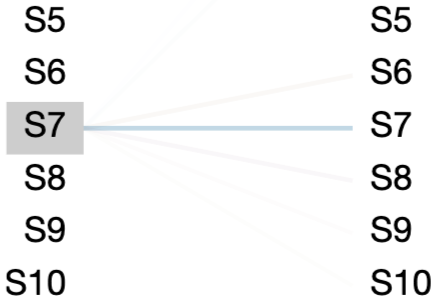
\includegraphics[width=\textwidth]{sec9-fig1.png}
%         \vspace{-6pt}
         \caption{Rel. from S7}
         \label{fig:stmt-7}
     \end{subfigure}
     \hfill
     \begin{subfigure}[b]{0.15\textwidth}
         \centering
         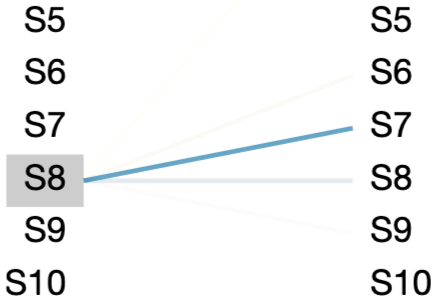
\includegraphics[width=\textwidth]{sec9-fig2.png}
%         \vspace{-6pt}
         \caption{Rel. from S8}
         \label{fig:stmt-8}
     \end{subfigure}
     \hfill
     \begin{subfigure}[b]{0.15\textwidth}
         \centering
         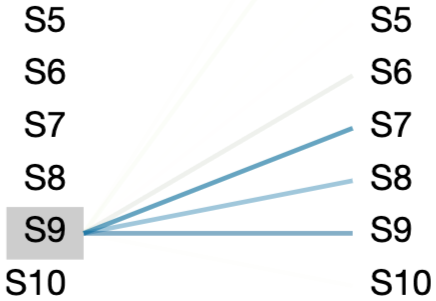
\includegraphics[width=\textwidth]{sec9-fig3.png}
%         \vspace{-6pt}
         \caption{Rel. from S9}
         \label{fig:stmt-9}
     \end{subfigure}
     \vspace{-9pt}
        \caption{Dependency Probing via Attentions for Figure~\ref{fig:rq1-case}}
        \label{fig:rq4-attention}
\end{figure}


\subsubsection{Distances between Statement Embeddings}
The confidence interval of the mean of cosine distances for the inside
statement group is from 0.1262 to 0.1268 with 95\% confidence, and the
confidence interval for the inside-to-outside statement group is
from 0.7987 to 0.8001 with 95\% confidence. As seen in
Figure~\ref{fig:rq4-density}, the distribution of the cosine distances
for all the inside-to-outside statement pairs is largely to the right
of the distribution for all the inside statement pairs. That is,
{\tool} tends to {\em encode statements in a way that the statements
  in the same \code{try} block are closer to each other in the
  embedding space}, leading to better grouping of statements.
  
\begin{figure}[t]
 	\centering
 	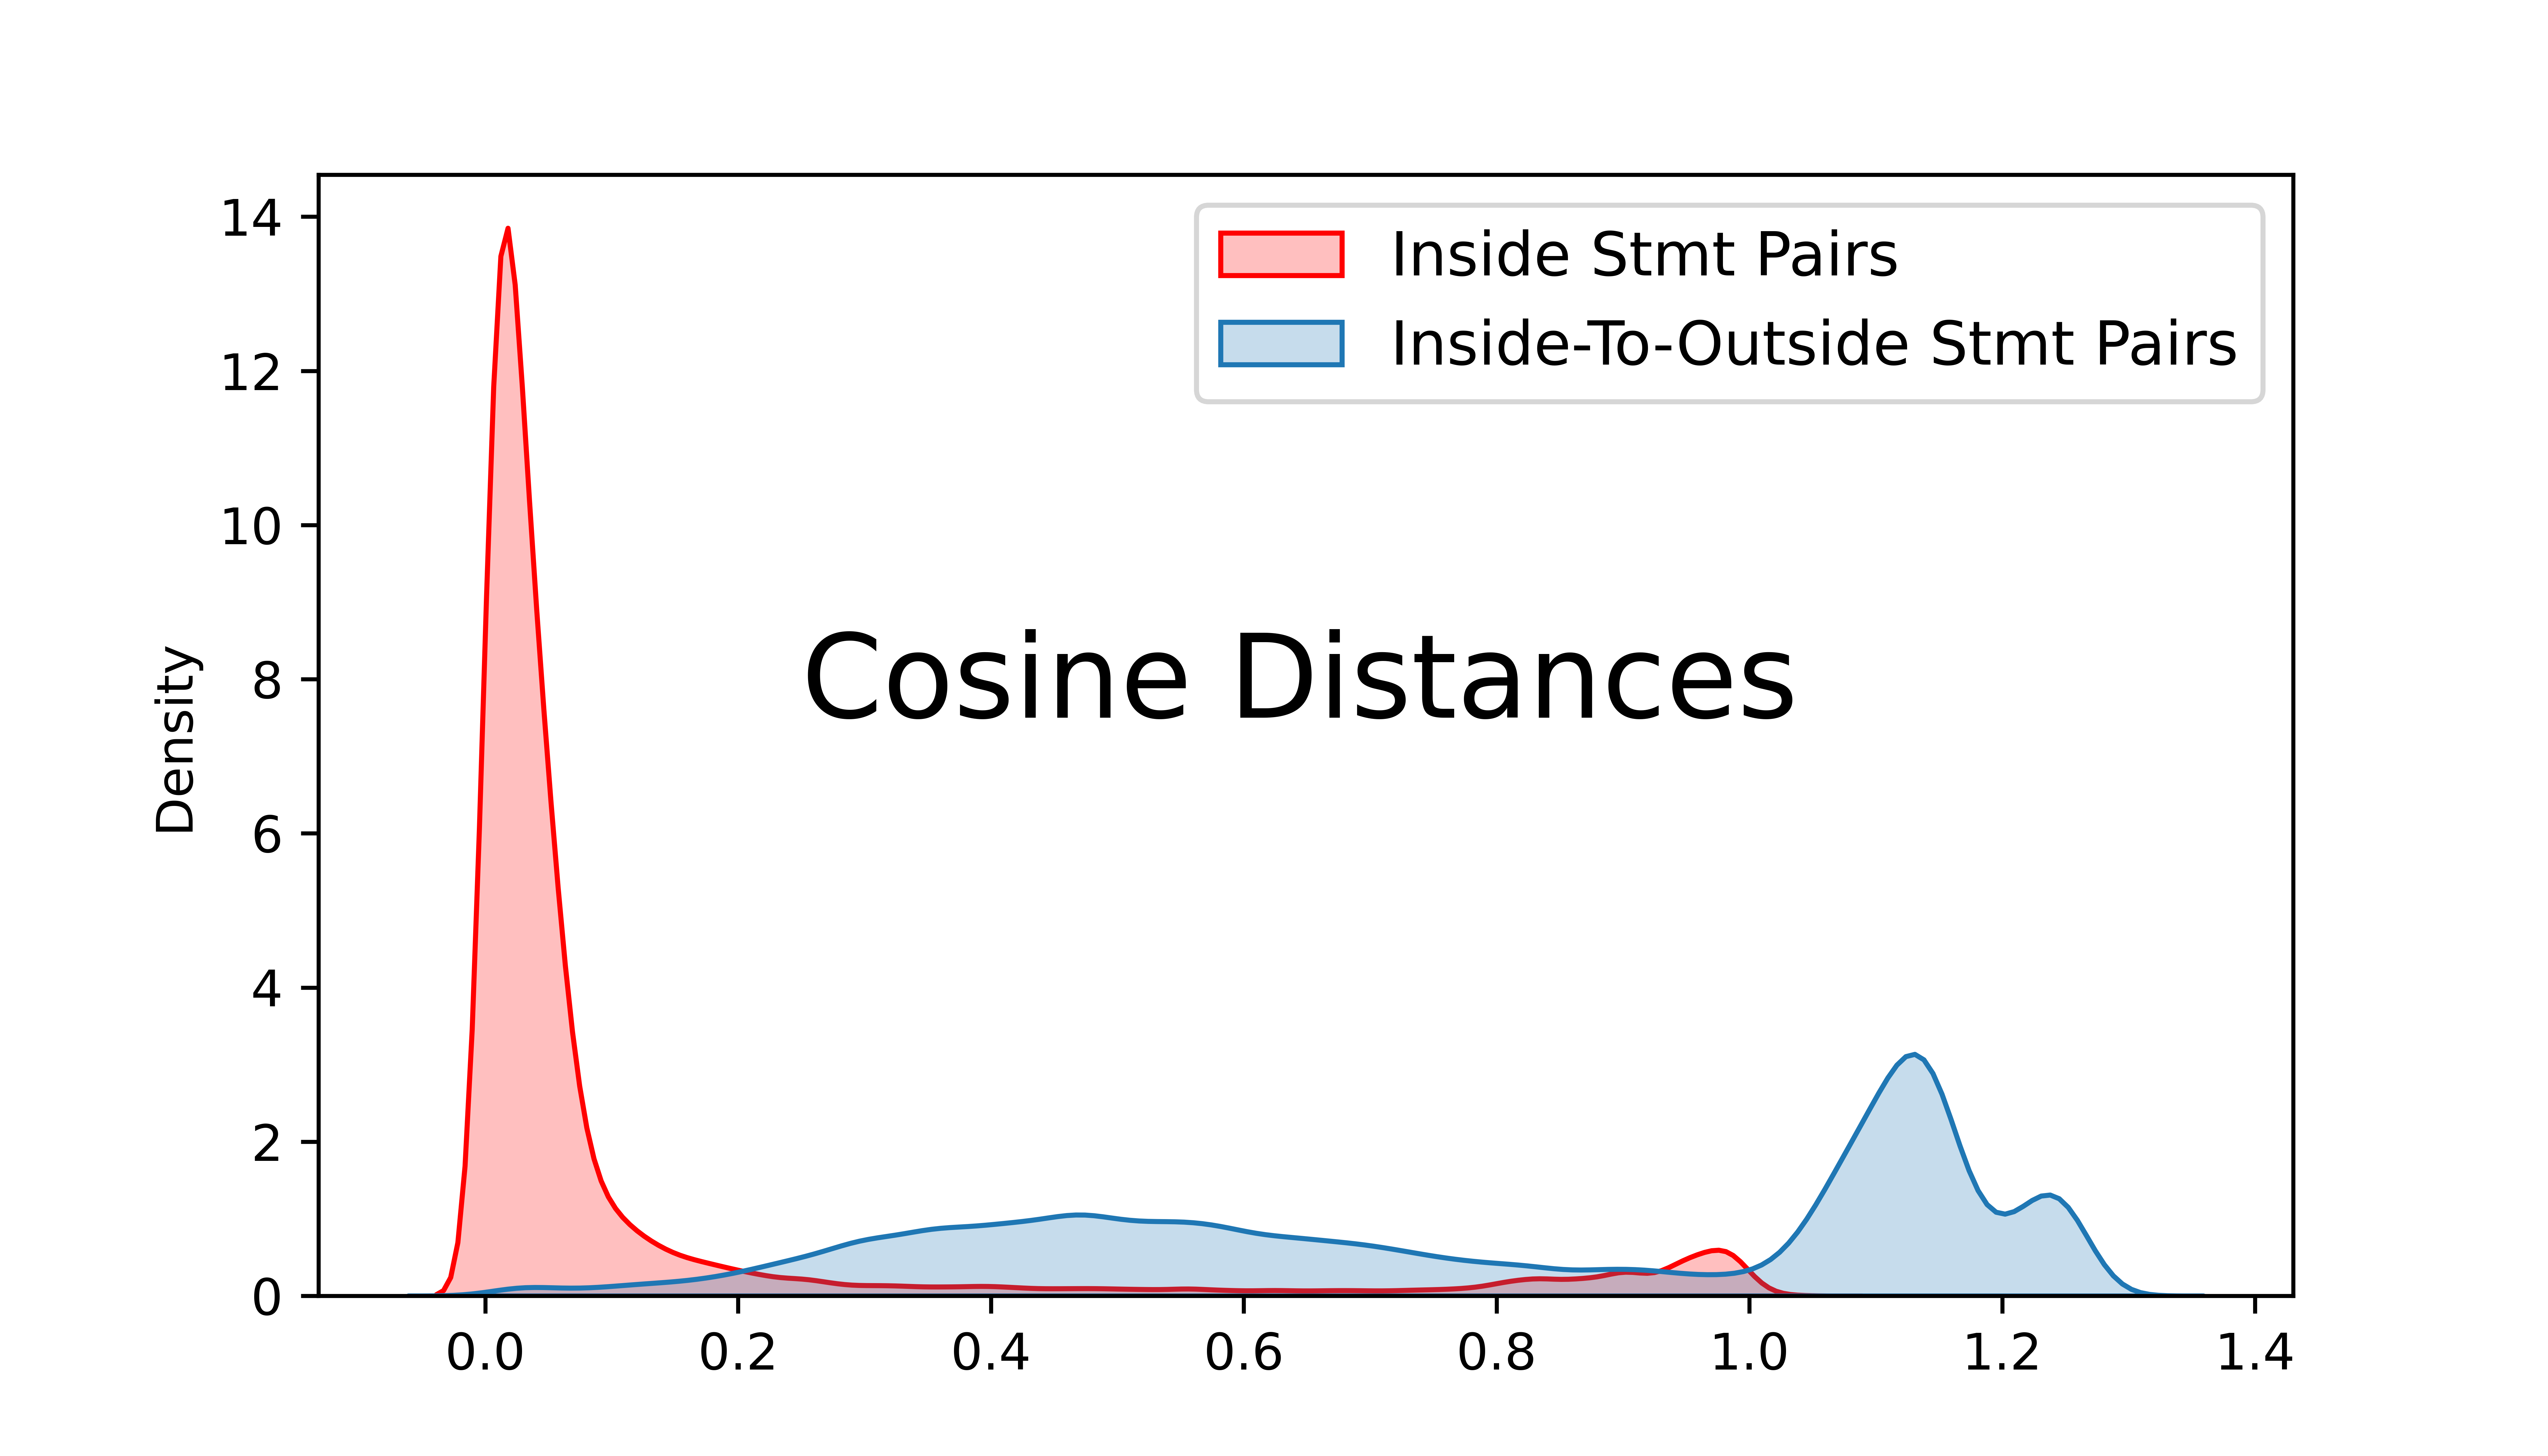
\includegraphics[width=2.6in]{rq4-density-v2.png}
        \vspace{-12pt}
 	\caption{Distribution of Cosine Distances}
 	\label{fig:rq4-density}	
\end{figure}




